\subsection{Robustness to prediction errors}\label{sec:res_robust}

Theorem~\ref{thm:carma} predicts that CARMA degrades gracefully as its predictions deteriorate. We test this on every fourth test week of 2024 (13 weeks, $\rho=0.5$, migration allowed, fresh workload seeds) by injecting controlled errors into the two kinds of prediction (Fig.~\ref{fig:robust}).

\begin{figure}[t]
\centering
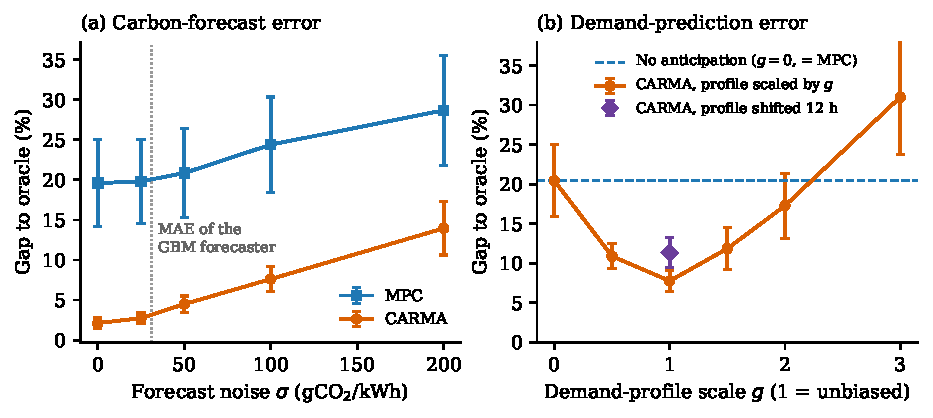
\includegraphics[width=\textwidth]{../figures/fig8_robust.pdf}
\caption{Graceful degradation under controlled prediction errors (13 test weeks of 2024, $\rho=0.5$, migration allowed; means with 95\% confidence intervals). (a) Carbon-intensity forecasts replaced by the realised values plus Gaussian noise of standard deviation $\sigma$. (b) Demand profile scaled by $g$, or shifted by 12 hours so that arrivals are predicted at the wrong time of day.}
\label{fig:robust}
\end{figure}

\paragraph{Carbon-forecast error} The forecasts were replaced by the realised intensities plus independent Gaussian noise of standard deviation $\sigma$. CARMA's gap to the oracle increases smoothly and almost linearly, from 2.1\% with exact forecasts to 2.7\%, 4.5\%, 7.6\% and 14.0\% at $\sigma=25$, 50, 100 and 200~gCO$_2$/kWh. The largest level is more than six times the MAE of the GBM forecaster. MPC starts from 19.6\% and rises to 28.7\%. Even with the noisiest forecasts, CARMA outperforms MPC with perfect forecasts, which confirms the ordering implied by Theorems~\ref{thm:lb} and~\ref{thm:carma}.

\paragraph{Demand-prediction error} Scaling the learned demand profile by $g$ produces a V-shaped response with its minimum at the unbiased profile ($g=1$, gap 7.8\%). Under-prediction by half ($g=0.5$) and over-prediction by half ($g=1.5$) cost 3.1 and 4.1 percentage points. Predicting arrivals at the wrong time of day (a 12-hour shift) costs 3.6 points. Removing anticipation ($g=0$) returns the MPC level (20.4\%). Only gross over-prediction ($g=3$, triple the true demand) is worse than no anticipation (31.0\%), because it makes CARMA hold clean capacity for work that never arrives. Late work was negligible in all 221 runs (at most 0.008\% of work). This is consistent with the robustness part of Theorem~\ref{thm:carma}: mispredictions change which capacity is used, but not whether deadlines are met. The largest ratio of CARMA's emissions to the oracle's over all runs was 1.52, far below the worst-case bound $\theta$.

\subsection{Fair carbon attribution}\label{sec:res_fair}

We evaluate Theorem~\ref{thm:core} on the 52 test weeks at $\rho=0.5$, treating the four sites as players. For every week and each of the 15 coalitions, we compute the hindsight value $c(C)$, and we also run CARMA with only the coalition's sites and jobs. Pooling pays: the hindsight optimum of the grand coalition emits 3.37~tCO$_2$ per week, against 6.70 for the four sites operating separately. With CARMA the figures are 3.63 against 6.88. The question is how to share the reduction. We compare three attributions. The \emph{location-based} attribution charges each site the emissions of its own jobs wherever they ran. The \emph{work-proportional} attribution splits the total in proportion to submitted work. The \emph{dual} attribution is Eq.~(\ref{eq:phi}). For CARMA's realised emissions, the dual attribution is applied to the hindsight value, and the online excess over the hindsight optimum is split in proportion to work. A check is violated when a coalition is charged more than it would emit on its own.

\begin{table}[t]
\centering
\caption{Coalitional stability of carbon attributions (52 test weeks of 2024, $\rho=0.5$). Coalition checks: share of the $52\times14$ (week, proper coalition) pairs in which the coalition is charged more than its stand-alone emissions. Weeks: share of weeks with at least one violation. IR: share of (week, site) pairs in which a site is charged more than its stand-alone emissions. Max.\ excess: largest violation (tCO$_2$).}
\label{tab:fair}
\footnotesize
\resizebox{\textwidth}{!}{%
\begin{tabular}{llrrrr}
\toprule
Benchmark & Attribution & Coalition checks (\%) & Weeks (\%) & IR (\%) & Max.\ excess \\
\midrule
\inputtable{../results/table_fair.tex}
\bottomrule
\end{tabular}}
\end{table}

Table~\ref{tab:fair} and Fig.~\ref{fig:fair} report the results. In the hindsight game, the dual attribution satisfies every one of the 728 coalition checks, as Theorem~\ref{thm:core} guarantees. The location-based and work-proportional attributions violate 46\% and 44\% of the checks and fail in every week. The location-based rule is individually irrational for South Scotland in all 52 weeks and for North West England in 51. Their own jobs are displaced to dirtier capacity by imported work, so under that rule they are charged more than they would emit on their own. The dual attribution resolves this by crediting the clean sites for the capacity they contribute. South Scotland receives a net credit of 0.91~tCO$_2$ per week and North West England is close to neutral, while London's charge (2.81~t) remains well below its stand-alone emissions (3.91~t). With CARMA's realised emissions, which is the practical case, the adjusted dual attribution remains individually rational for every site in every week. It violates only 5 of the 728 coalition checks, with a largest excess of 0.06~tCO$_2$, whereas the location-based and work-proportional rules again fail in 43\% of the checks. Stand-alone coalitions occasionally leave a little work late (at most 4.7\%), and unfinished work emits nothing, so the online checks, if anything, favour secession.

\begin{figure}[t]
\centering
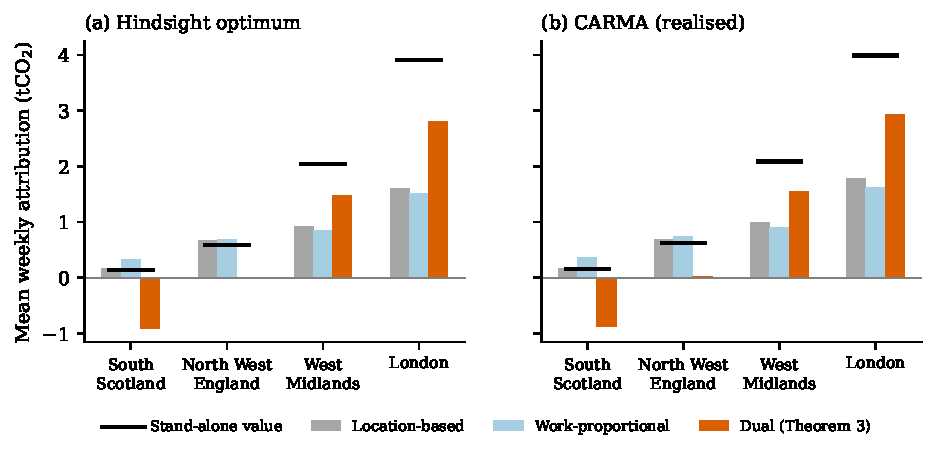
\includegraphics[width=\textwidth]{../figures/fig9_fairness.pdf}
\caption{Mean weekly carbon attribution by site under three rules, compared with each site's stand-alone emissions (black bars), 52 test weeks of 2024 at $\rho=0.5$. (a) Hindsight optimum. (b) CARMA's realised emissions. Negative values are net credits for contributing low-carbon capacity.}
\label{fig:fair}
\end{figure}
